\documentclass{ximera}

%\usepackage{todonotes}

\newcommand{\todo}{}

\usepackage{esint} % for \oiint
\ifxake%%https://math.meta.stackexchange.com/questions/9973/how-do-you-render-a-closed-surface-double-integral
\renewcommand{\oiint}{{\large\bigcirc}\kern-1.56em\iint}
\fi


\graphicspath{
  {./}
  {ximeraTutorial/}
  {basicPhilosophy/}
  {functionsOfSeveralVariables/}
  {normalVectors/}
  {lagrangeMultipliers/}
  {vectorFields/}
  {greensTheorem/}
  {shapeOfThingsToCome/}
  {dotProducts/}
  {partialDerivativesAndTheGradientVector/}
  {../productAndQuotientRules/exercises/}
  {../normalVectors/exercisesParametricPlots/}
  {../continuityOfFunctionsOfSeveralVariables/exercises/}
  {../partialDerivativesAndTheGradientVector/exercises/}
  {../directionalDerivativeAndChainRule/exercises/}
  {../commonCoordinates/exercisesCylindricalCoordinates/}
  {../commonCoordinates/exercisesSphericalCoordinates/}
  {../greensTheorem/exercisesCurlAndLineIntegrals/}
  {../greensTheorem/exercisesDivergenceAndLineIntegrals/}
  {../shapeOfThingsToCome/exercisesDivergenceTheorem/}
  {../greensTheorem/}
  {../shapeOfThingsToCome/}
  {../separableDifferentialEquations/exercises/}
  {vectorFields/}
}

\newcommand{\mooculus}{\textsf{\textbf{MOOC}\textnormal{\textsf{ULUS}}}}

\usepackage{tkz-euclide}
\usepackage{tikz}
\usepackage{tikz-cd}
\usetikzlibrary{arrows}
\tikzset{>=stealth,commutative diagrams/.cd,
  arrow style=tikz,diagrams={>=stealth}} %% cool arrow head
\tikzset{shorten <>/.style={ shorten >=#1, shorten <=#1 } } %% allows shorter vectors

\usetikzlibrary{backgrounds} %% for boxes around graphs
\usetikzlibrary{shapes,positioning}  %% Clouds and stars
\usetikzlibrary{matrix} %% for matrix
\usepgfplotslibrary{polar} %% for polar plots
\usepgfplotslibrary{fillbetween} %% to shade area between curves in TikZ
%\usetkzobj{all}
\usepackage[makeroom]{cancel} %% for strike outs
%\usepackage{mathtools} %% for pretty underbrace % Breaks Ximera
%\usepackage{multicol}
\usepackage{pgffor} %% required for integral for loops



%% http://tex.stackexchange.com/questions/66490/drawing-a-tikz-arc-specifying-the-center
%% Draws beach ball
\tikzset{pics/carc/.style args={#1:#2:#3}{code={\draw[pic actions] (#1:#3) arc(#1:#2:#3);}}}



\usepackage{array}
\setlength{\extrarowheight}{+.1cm}
\newdimen\digitwidth
\settowidth\digitwidth{9}
\def\divrule#1#2{
\noalign{\moveright#1\digitwidth
\vbox{\hrule width#2\digitwidth}}}




% \newcommand{\RR}{\mathbb R}
% \newcommand{\R}{\mathbb R}
% \newcommand{\N}{\mathbb N}
% \newcommand{\Z}{\mathbb Z}

\newcommand{\sagemath}{\textsf{SageMath}}


%\renewcommand{\d}{\,d\!}
%\renewcommand{\d}{\mathop{}\!d}
%\newcommand{\dd}[2][]{\frac{\d #1}{\d #2}}
%\newcommand{\pp}[2][]{\frac{\partial #1}{\partial #2}}
% \renewcommand{\l}{\ell}
%\newcommand{\ddx}{\frac{d}{\d x}}

% \newcommand{\zeroOverZero}{\ensuremath{\boldsymbol{\tfrac{0}{0}}}}
%\newcommand{\inftyOverInfty}{\ensuremath{\boldsymbol{\tfrac{\infty}{\infty}}}}
%\newcommand{\zeroOverInfty}{\ensuremath{\boldsymbol{\tfrac{0}{\infty}}}}
%\newcommand{\zeroTimesInfty}{\ensuremath{\small\boldsymbol{0\cdot \infty}}}
%\newcommand{\inftyMinusInfty}{\ensuremath{\small\boldsymbol{\infty - \infty}}}
%\newcommand{\oneToInfty}{\ensuremath{\boldsymbol{1^\infty}}}
%\newcommand{\zeroToZero}{\ensuremath{\boldsymbol{0^0}}}
%\newcommand{\inftyToZero}{\ensuremath{\boldsymbol{\infty^0}}}



% \newcommand{\numOverZero}{\ensuremath{\boldsymbol{\tfrac{\#}{0}}}}
% \newcommand{\dfn}{\textbf}
% \newcommand{\unit}{\,\mathrm}
% \newcommand{\unit}{\mathop{}\!\mathrm}
% \newcommand{\eval}[1]{\bigg[ #1 \bigg]}
% \newcommand{\seq}[1]{\left( #1 \right)}
% \renewcommand{\epsilon}{\varepsilon}
% \renewcommand{\phi}{\varphi}


% \renewcommand{\iff}{\Leftrightarrow}

% \DeclareMathOperator{\arccot}{arccot}
% \DeclareMathOperator{\arcsec}{arcsec}
% \DeclareMathOperator{\arccsc}{arccsc}
% \DeclareMathOperator{\si}{Si}
% \DeclareMathOperator{\scal}{scal}
% \DeclareMathOperator{\sign}{sign}


%% \newcommand{\tightoverset}[2]{% for arrow vec
%%   \mathop{#2}\limits^{\vbox to -.5ex{\kern-0.75ex\hbox{$#1$}\vss}}}
% \newcommand{\arrowvec}[1]{{\overset{\rightharpoonup}{#1}}}
% \renewcommand{\vec}[1]{\arrowvec{\mathbf{#1}}}
% \renewcommand{\vec}[1]{{\overset{\boldsymbol{\rightharpoonup}}{\mathbf{#1}}}}

% \newcommand{\point}[1]{\left(#1\right)} %this allows \vector{ to be changed to \vector{ with a quick find and replace
% \newcommand{\pt}[1]{\mathbf{#1}} %this allows \vec{ to be changed to \vec{ with a quick find and replace
% \newcommand{\Lim}[2]{\lim_{\point{#1} \to \point{#2}}} %Bart, I changed this to point since I want to use it.  It runs through both of the exercise and exerciseE files in limits section, which is why it was in each document to start with.

% \DeclareMathOperator{\proj}{\mathbf{proj}}
% \newcommand{\veci}{{\boldsymbol{\hat{\imath}}}}
% \newcommand{\vecj}{{\boldsymbol{\hat{\jmath}}}}
% \newcommand{\veck}{{\boldsymbol{\hat{k}}}}
% \newcommand{\vecl}{\vec{\boldsymbol{\l}}}
% \newcommand{\uvec}[1]{\mathbf{\hat{#1}}}
% \newcommand{\utan}{\mathbf{\hat{t}}}
% \newcommand{\unormal}{\mathbf{\hat{n}}}
% \newcommand{\ubinormal}{\mathbf{\hat{b}}}

% \newcommand{\dotp}{\bullet}
% \newcommand{\cross}{\boldsymbol\times}
% \newcommand{\grad}{\boldsymbol\nabla}
% \newcommand{\divergence}{\grad\dotp}
% \newcommand{\curl}{\grad\cross}
%\DeclareMathOperator{\divergence}{divergence}
%\DeclareMathOperator{\curl}[1]{\grad\cross #1}
% \newcommand{\lto}{\mathop{\longrightarrow\,}\limits}

% \renewcommand{\bar}{\overline}

\colorlet{textColor}{black}
\colorlet{background}{white}
\colorlet{penColor}{blue!50!black} % Color of a curve in a plot
\colorlet{penColor2}{red!50!black}% Color of a curve in a plot
\colorlet{penColor3}{red!50!blue} % Color of a curve in a plot
\colorlet{penColor4}{green!50!black} % Color of a curve in a plot
\colorlet{penColor5}{orange!80!black} % Color of a curve in a plot
\colorlet{penColor6}{yellow!70!black} % Color of a curve in a plot
\colorlet{fill1}{penColor!20} % Color of fill in a plot
\colorlet{fill2}{penColor2!20} % Color of fill in a plot
\colorlet{fillp}{fill1} % Color of positive area
\colorlet{filln}{penColor2!20} % Color of negative area
\colorlet{fill3}{penColor3!20} % Fill
\colorlet{fill4}{penColor4!20} % Fill
\colorlet{fill5}{penColor5!20} % Fill
\colorlet{gridColor}{gray!50} % Color of grid in a plot

\newcommand{\surfaceColor}{violet}
\newcommand{\surfaceColorTwo}{redyellow}
\newcommand{\sliceColor}{greenyellow}




\pgfmathdeclarefunction{gauss}{2}{% gives gaussian
  \pgfmathparse{1/(#2*sqrt(2*pi))*exp(-((x-#1)^2)/(2*#2^2))}%
}


%%%%%%%%%%%%%
%% Vectors
%%%%%%%%%%%%%

%% Simple horiz vectors
\renewcommand{\vector}[1]{\left\langle #1\right\rangle}


%% %% Complex Horiz Vectors with angle brackets
%% \makeatletter
%% \renewcommand{\vector}[2][ , ]{\left\langle%
%%   \def\nextitem{\def\nextitem{#1}}%
%%   \@for \el:=#2\do{\nextitem\el}\right\rangle%
%% }
%% \makeatother

%% %% Vertical Vectors
%% \def\vector#1{\begin{bmatrix}\vecListA#1,,\end{bmatrix}}
%% \def\vecListA#1,{\if,#1,\else #1\cr \expandafter \vecListA \fi}

%%%%%%%%%%%%%
%% End of vectors
%%%%%%%%%%%%%

%\newcommand{\fullwidth}{}
%\newcommand{\normalwidth}{}



%% makes a snazzy t-chart for evaluating functions
%\newenvironment{tchart}{\rowcolors{2}{}{background!90!textColor}\array}{\endarray}

%%This is to help with formatting on future title pages.
\newenvironment{sectionOutcomes}{}{}



%% Flowchart stuff
%\tikzstyle{startstop} = [rectangle, rounded corners, minimum width=3cm, minimum height=1cm,text centered, draw=black]
%\tikzstyle{question} = [rectangle, minimum width=3cm, minimum height=1cm, text centered, draw=black]
%\tikzstyle{decision} = [trapezium, trapezium left angle=70, trapezium right angle=110, minimum width=3cm, minimum height=1cm, text centered, draw=black]
%\tikzstyle{question} = [rectangle, rounded corners, minimum width=3cm, minimum height=1cm,text centered, draw=black]
%\tikzstyle{process} = [rectangle, minimum width=3cm, minimum height=1cm, text centered, draw=black]
%\tikzstyle{decision} = [trapezium, trapezium left angle=70, trapezium right angle=110, minimum width=3cm, minimum height=1cm, text centered, draw=black]


\title{Two Sides}

\begin{document}

\begin{abstract}
both sides together
\end{abstract}
\maketitle



Tangent lines are lines that are tangent to a curve or graph at a tangent point. There must be a point on the curve. At that tangent point, the curve or graph is behaving in some manner, which the tangent line is modeling.  \\

\begin{idea} \textbf{\textcolor{blue!55!black}{Tangent Line}}


A tangent line is a line that does the best job of pretending to be the curve at a single point.
\end{idea}


\textbf{Best job} means the line shares the tangent point with the curve and the slope of the line is the same as the ``slope'' of the curve at the tangent point. \\

If you zoomed in on the graph at the tangent point, then the curve would slowly begin to look just like the line. \\


For quadratics, we have a formula for the $iRoC$ or derivative, which gives the exact slope of each tangent line along the parabola.  But, for a random function, how do you get a tangent line for its graph without knowing the slope ahead of time? \\


We are returning to our idea of a secant line and moving it over to a tangent point. \\

\textbf{\textcolor{red!90!darkgray}{$\blacktriangleright$}} There are two behaviors happening as we shift a secant line. One behavior of the graph and one behavior attached to the secant lines. The graph is behaviing and the secant lines are behaving. \\



\begin{itemize}
\item \textbf{First}, the curve or graph itself is approaching that point, from both sides. The graph is connecting up to the point. There is no break. The function is continuous at the corresponding domain number.\\
\item \textbf{Second}, the secant lines are smoothly turning into the tangent line at the tangent point. \\
\end{itemize}



\begin{warning} \textbf{\textcolor{red!80!black}{Both Sides}}

This means both sides of the tangent point. \\

The graph points on both sides are approaching the tangent point. \\

The secant lines on both sides are approaching the tangent line.

\end{warning}
\textbf{Later}, we will also consider the situation where the graph only has one side. \\





\begin{idea}   \textbf{\textcolor{blue!55!black}{Special Secant Lines}}


To help us watch the moving secant lines, we are going to use special secant lines. \\

We are using secant lines that also go through the tangent point. \\

We need two points on the graph for a secant. One of the points will be the tangent point.  The second point will be another point on the graph. \\

To move the secant line, we will select graph points that are getting ever closer to the tangent point. \\

We can do this on either side of the tangent line. \\

This will help our eyes.


\end{idea}


\textbf{Note:} We are considering the situation where we have both sides, which means the domain number corresponding to the tangent line is inside an open interval in the domain. \\













\subsection*{Two Sides : Points and Secants Agree}


The setup: \\

\begin{itemize}
     \item Let $f(t)$ be a function and $t_0$ a domain number. \\

     \item $t_0$ is inside an open interval in the domain, $t_0 \in (a, b) \subset Domain$. (Because, we need two sides.) \\

     \item The graph point $(t_0 , f(t_0))$ is our tangent point on the graph.
\end{itemize}


Our secant lines are special secant lines. Rather than a secant line running through two points on either side of the tangent point, our secant lines will use the tangent point as one of its points. \\ 



Suppose the points on the graph approach the point $(t_0 , f(t_0))$ and the secant lines (from both sides) approach the same line.



\textbf{\textcolor{blue!55!black}{Example}}  \\




Here is the graph of the function $f(x) = (x - 3)^2 - 4$ and the point $(4, f(4))= (4, -3)$. \\

\begin{image}
\begin{tikzpicture}
     \begin{axis}[
                domain=-10:10, ymax=10, xmax=10, ymin=-6, xmin=-6,
                axis lines =center, xlabel=$x$, ylabel=$y$,
                ytick={-6,-4,-2,2,4,6,8,10},
                xtick={-6,-4,-2,2,4,6,8,10},
                ticklabel style={font=\scriptsize},
                every axis y label/.style={at=(current axis.above origin),anchor=south},
                every axis x label/.style={at=(current axis.right of origin),anchor=west},
                axis on top,
                ]


        \addplot [draw=penColor, very thick, smooth, domain=(0:6),<->] {(x-3)^2 - 4};

        \addplot [color=penColor2,only marks,mark=*] coordinates{(4,-3)};
        


        %\node[penColor] at (axis cs:5,-4) {$(h, k)$};
        %\node[penColor] at (axis cs:5,-9) {$-0.5 x^2 - 5 x + 15.5$};



    \end{axis}
\end{tikzpicture}
\end{image}

A parabola and a point on the parabola. \\


\textbf{First}, the points on the graph are approaching the point $(4, -3)$ on both sides.  There is no break in the curve. $f$ is continuous at $4$.\\


The soon to be tangent point is $(4, -3)$ and a tangent line runs through it.\\







\begin{image}
\begin{tikzpicture}
     \begin{axis}[
                domain=-10:10, ymax=10, xmax=10, ymin=-6, xmin=-6,
                axis lines =center, xlabel=$x$, ylabel=$y$,
                ytick={-6,-4,-2,2,4,6,8,10},
                xtick={-6,-4,-2,2,4,6,8,10},
                ticklabel style={font=\scriptsize},
                every axis y label/.style={at=(current axis.above origin),anchor=south},
                every axis x label/.style={at=(current axis.right of origin),anchor=west},
                axis on top,
                ]


        \addplot [draw=penColor, very thick, smooth, domain=(0:6),<->] {(x-3)^2 - 4};

        \addplot [color=penColor,only marks,mark=*] coordinates{(4,-3)};
        
        \addplot [draw=penColor2, very thick, smooth, domain=(3:8),<->] {2*(x-4)-3};

        %\node[penColor] at (axis cs:5,-4) {$(h, k)$};
        %\node[penColor] at (axis cs:5,-9) {$-0.5 x^2 - 5 x + 15.5$};



    \end{axis}
\end{tikzpicture}
\end{image}



The tangent line does the best job of modeling the curve right at the tangent point. If you were to zoom in closely to the point $(4, -3)$, the line and the curve would look the same.\\


As it turns out, we know how to get the slope of lines tangent to a parabola.  Use the derivative of $f$ or $iRoC_f$.   

\[ 
f'(x)=iRoC_f(x) = 2 (x - 3)^2
\] 

In this example, the slope of this tangent line is $f'(3) = 2 (4-3)^2 = 2$ \\

Using the point-slope form of a line, we can get an equation for the tangent line, $y - (-3)=2 (x-4)$. That gives us a tangent line described by the equation $y = 2 (x - 4) - 3$.











\textbf{Second}, For every other point on the parabola, there is a line through that point and the tangent point.  These are called \textit{secant lines}. These secant lines run through approaching points and the tangent line. These secant lines smoothly turn into the tangent line at the tangent point...on both sides.


Here are the secant lines through the tangent point and the approaching points $(3, -4)$, $(3.3, -3.91)$, $(3.7, -3.51)$, $(4.3, -2.31)$, $(4.7, -1.11)$, and $(5, 0)$.



\begin{image}
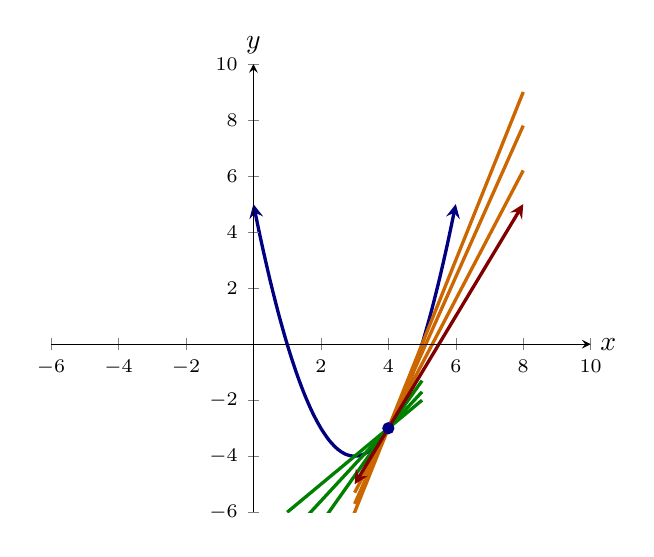
\begin{tikzpicture}
     \begin{axis}[
                domain=-10:10, ymax=10, xmax=10, ymin=-6, xmin=-6,
                axis lines =center, xlabel=$x$, ylabel=$y$,
                ytick={-6,-4,-2,2,4,6,8,10},
                xtick={-6,-4,-2,2,4,6,8,10},
                ticklabel style={font=\scriptsize},
                every axis y label/.style={at=(current axis.above origin),anchor=south},
                every axis x label/.style={at=(current axis.right of origin),anchor=west},
                axis on top,
                ]


        \addplot [draw=penColor, very thick, smooth, domain=(0:6),<->] {(x-3)^2 - 4};

        \addplot [color=penColor,only marks,mark=*] coordinates{(4,-3)};
        
       


        \addplot [draw=penColor4, very thick, smooth, domain=(1:5)] {(x-4)-3};
        \addplot [draw=penColor4, very thick, smooth, domain=(1:5)] {1.3*(x-4)-3};
        \addplot [draw=penColor4, very thick, smooth, domain=(1:5)] {1.7*(x-4)-3};

        \addplot [draw=penColor5, very thick, smooth, domain=(3:8)] {2.3*(x-4)-3};
        \addplot [draw=penColor5, very thick, smooth, domain=(3:8)] {2.7*(x-4)-3};
        \addplot [draw=penColor5, very thick, smooth, domain=(1:8)] {3*(x-4)-3};


          \addplot [draw=penColor2, very thick, smooth, domain=(3:8),<->] {2*(x-4)-3};



        %\node[penColor] at (axis cs:5,-4) {$(h, k)$};
        %\node[penColor] at (axis cs:5,-9) {$-0.5 x^2 - 5 x + 15.5$};



    \end{axis}
\end{tikzpicture}
\end{image}






\begin{image}
\begin{tikzpicture}
     \begin{axis}[
                domain=2:5.5, ymax=1, xmax=5.5, ymin=-4, xmin=2,
                axis lines =center, xlabel=$x$, ylabel=$y$,
                ytick={--4,-3,-2,-1,1},
                xtick={2,3,4,5},
                ticklabel style={font=\scriptsize},
                every axis y label/.style={at=(current axis.above origin),anchor=south},
                every axis x label/.style={at=(current axis.right of origin),anchor=west},
                axis on top,
                ]


        \addplot [draw=penColor, very thick, smooth, domain=(2:5.5),<->] {(x-3)^2 - 4};

        \addplot [color=penColor,only marks,mark=*] coordinates{(4,-3)};
        
       


        %\addplot [draw=penColor4, very thick, smooth, domain=(1:5)] {(x-4)-3};
        %\addplot [draw=penColor4, very thick, smooth, domain=(1:5)] {1.3*(x-4)-3};
        %\addplot [draw=penColor4, very thick, smooth, domain=(1:5)] {1.7*(x-4)-3};

        %\addplot [draw=penColor5, very thick, smooth, domain=(3:8)] {2.3*(x-4)-3};
        %\addplot [draw=penColor5, very thick, smooth, domain=(3:8)] {2.7*(x-4)-3};
        %\addplot [draw=penColor5, very thick, smooth, domain=(1:8)] {3*(x-4)-3};


        %\addplot [draw=penColor2, very thick, smooth, domain=(3:8),<->] {2*(x-4)-3};





    \end{axis}
\end{tikzpicture}
\end{image}






The secant lines on the left smootly turn into the tangent line as you move to the right. The secant lines on the right smoothly turn into the tangent line as you move to the left. \\






























\subsection*{Two Sides : Points Agree and Secants Disagree}


Suppose our tangent point is $(t_0 , f(t_0))$ and $t_0$ is inside an open interval in the domain, $t_0 \in (a, b) \subset Domain$. \\


Suppose the points on the graph approach the point $(t_0 , f(t_0))$, however the secant lines (from both sides) do not approach the same line.



\textbf{\textcolor{blue!55!black}{Example}}  \\




Here is the graph of the function $f(x) = | x - 3 | - 4$ and the point $(3, f(3))= (3, -4)$. \\

\begin{image}
\begin{tikzpicture}
     \begin{axis}[
                domain=-10:10, ymax=10, xmax=10, ymin=-6, xmin=-6,
                axis lines =center, xlabel=$x$, ylabel=$y$,
                ytick={-6,-4,-2,2,4,6,8,10},
                xtick={-6,-4,-2,2,4,6,8,10},
                ticklabel style={font=\scriptsize},
                every axis y label/.style={at=(current axis.above origin),anchor=south},
                every axis x label/.style={at=(current axis.right of origin),anchor=west},
                axis on top,
                ]

        \addplot [draw=penColor, very thick, smooth, domain=(3:9),->] {x-7};
        \addplot [draw=penColor, very thick, smooth, domain=(-5:3),<-] {-x-1};

        \addplot [color=penColor2,only marks,mark=*] coordinates{(3,-4)};
        


        %\node[penColor] at (axis cs:5,-4) {$(h, k)$};
        %\node[penColor] at (axis cs:5,-9) {$-0.5 x^2 - 5 x + 15.5$};



    \end{axis}
\end{tikzpicture}
\end{image}

An absolute value ``Vee'' and its corner point. \\


\textbf{First}, the points on the graph are approaching the point on both sides.  There is no break in the curve. $f$ is continuous at $3$.\\


The hopeful tangent point is $(3, -4)$ \\


If there is a tangent line, then the secant lines should smoothly turn into the tangent line, on both sides.  \\


The other way of thinking of this is that if the secant lines on both sides do not smoothly turn into the same line, then there cannot be a tangent line. \\

That is the case here. \\








\textbf{Second}, the secant lines lines through approaching points do not smoothly turn into the tangent line at the tangent point...on both sides.


Here are the secant lines through the tangent point and the approaching points $(2, -3)$, $(2.3, -3.3)$, $(2.7, -3.7)$, $(3.3, -3.7)$, $(3.7, -3.3)$, and $(4, -3)$.





\begin{image}
\begin{tikzpicture}
     \begin{axis}[
                domain=-10:10, ymax=10, xmax=10, ymin=-6, xmin=-6,
                axis lines =center, xlabel=$x$, ylabel=$y$,
                ytick={-6,-4,-2,2,4,6,8,10},
                xtick={-6,-4,-2,2,4,6,8,10},
                ticklabel style={font=\scriptsize},
                every axis y label/.style={at=(current axis.above origin),anchor=south},
                every axis x label/.style={at=(current axis.right of origin),anchor=west},
                axis on top,
                ]


          \addplot [draw=penColor, very thick, smooth, domain=(3:9),->] {(x-7)};
        \addplot [draw=penColor, very thick, smooth, domain=(-5:3),<-] {(-x-1)};

          \addplot [color=penColor2,only marks,mark=*] coordinates{(3,-4)};
        
          \addplot [draw=penColor4, very thick, smooth, domain=(0:5)] {-1*(x-3)-4};

          \addplot [draw=penColor5, very thick, smooth, domain=(2:6)] {(x-3)-4};



    \end{axis}
\end{tikzpicture}
\end{image}






The secant lines on the left smootly turn into a line as you move to the right. The secant lines on the right smoothly turn into a line as you move to the left. \\

\textbf{\textcolor{blue!55!black}{BUT!  They are NOT the same line!}}\\


There is no common line that the secand lines are approaching. \\

There is no tangent line at the pont $(3,-4)$. \\

There is no slope of a tangent line. \\

$f$ has no derivative value at $3$.  \\

$f'(3)$ does not exist. \\

$3$ is a number in the domain, but $f'(3)$ does not exist. \\

($3$ is a critical number.)

































\section*{Two Sides : Points Agree and Secants Agree, but No Slope}


Suppose our tangent point is $(t_0 , f(t_0))$ and $t_0$ is inside an open interval in the domain, $t_0 \in (a, b) \subset Domain$. \\


Suppose the points on the graph approach the point $(t_0 , f(t_0))$, and the secant lines (from both sides) approach the same line, but it is a vertical line. \\



\textbf{\textcolor{blue!55!black}{Example}}  \\




Here is the graph of the function $f(x) = 4 \, \sqrt[3]{x-2}$ and the point $(2, f(2))= (2, 0)$. \\

\begin{image}
\begin{tikzpicture}
     \begin{axis}[
                domain=-10:10, ymax=10, xmax=10, ymin=-10, xmin=-10,
                axis lines =center, xlabel=$x$, ylabel=$y$,
                ytick={-10,-8,-6,-4,-2,2,4,6,8,10},
                xtick={-10,-8,-6,-4,-2,2,4,6,8,10},
                ticklabel style={font=\scriptsize},
                every axis y label/.style={at=(current axis.above origin),anchor=south},
                every axis x label/.style={at=(current axis.right of origin),anchor=west},
                axis on top,
                ]


        \addplot [draw=penColor, very thick, smooth, samples=300, domain=(2:9),->] {4*(x-2)^(0.3333)};
        \addplot [draw=penColor, very thick, smooth, samples=300, domain=(-5:2),<-] {-4*(2-x)^(0.3333)};

        \addplot [color=penColor2,only marks,mark=*] coordinates{(2,0)};
        




    \end{axis}
\end{tikzpicture}
\end{image}

A cube root and a point on the graph. \\











\textbf{First}, the points on the graph are approaching the point on both sides.  There is no break in the curve. $f$ is continuous at $3$.\\


The hopeful tangent point is $(2, 0)$ \\

There is a tangent line.\\




\begin{image}
\begin{tikzpicture}
     \begin{axis}[
                domain=-10:10, ymax=10, xmax=10, ymin=-10, xmin=-10,
                axis lines =center, xlabel=$x$, ylabel=$y$,
                ytick={-10,-8,-6,-4,-2,2,4,6,8,10},
                xtick={-10,-8,-6,-4,-2,2,4,6,8,10},
                ticklabel style={font=\scriptsize},
                every axis y label/.style={at=(current axis.above origin),anchor=south},
                every axis x label/.style={at=(current axis.right of origin),anchor=west},
                axis on top,
                ]


        \addplot [draw=penColor, very thick, smooth, samples=300, domain=(2:9),->] {4*(x-2)^(0.3333)};
        \addplot [draw=penColor, very thick, smooth, samples=300, domain=(-5:2),<-] {-4*(2-x)^(0.3333)};

        \addplot [color=penColor2,only marks,mark=*] coordinates{(2,0)};
        

          \addplot [line width=1, penColor2, smooth,samples=200,domain=(-6:6)] ({2},{x});


    \end{axis}
\end{tikzpicture}
\end{image}












The tangent line does the best job of modeling the curve right at the tangent point. \\

Here, the tangent line is described by the equation $x = 2$. It is a vertical line. \\











\textbf{Second}, the secant lines lines through approaching points smoothly turn into the tangent line at the tangent point...on both sides.


Here are the secant lines through the tangent point and the approaching points $(1, -4)$, $(1.3, -3.91)$, $(1.7, -3.51)$, $(2.3, -2.31)$, $(2.7, -1.11)$, and $(3, 0)$.



\begin{image}
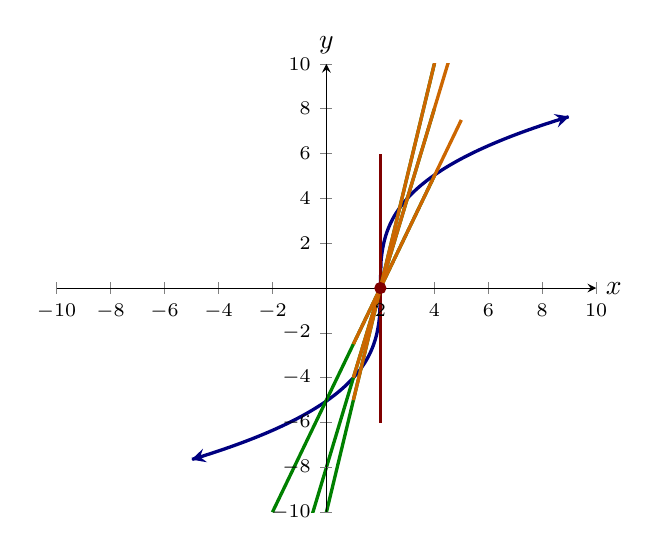
\begin{tikzpicture}
     \begin{axis}[
                domain=-10:10, ymax=10, xmax=10, ymin=-10, xmin=-10,
                axis lines =center, xlabel=$x$, ylabel=$y$,
                ytick={-10,-8,-6,-4,-2,2,4,6,8,10},
                xtick={-10,-8,-6,-4,-2,2,4,6,8,10},
                ticklabel style={font=\scriptsize},
                every axis y label/.style={at=(current axis.above origin),anchor=south},
                every axis x label/.style={at=(current axis.right of origin),anchor=west},
                axis on top,
                ]



         \addplot [draw=penColor, very thick, smooth, samples=300, domain=(2:9),->] {4*(x-2)^(0.3333)};
        \addplot [draw=penColor, very thick, smooth, samples=300, domain=(-5:2),<-] {-4*(2-x)^(0.3333)};

        \addplot [color=penColor2,only marks,mark=*] coordinates{(2,0)};
        

          \addplot [line width=1, penColor2, smooth,samples=200,domain=(-6:6)] ({2},{x});
        
       


        \addplot [draw=penColor4, very thick, smooth, domain=(-2:4)] {2.5*(x-2)};
        \addplot [draw=penColor4, very thick, smooth, domain=(-2:4)] {4*(x-2)};
        \addplot [draw=penColor4, very thick, smooth, domain=(-2:4)] {5*(x-2)};

        \addplot [draw=penColor5, very thick, smooth, domain=(1:5)] {5*(x-2)};
        \addplot [draw=penColor5, very thick, smooth, domain=(1:5)] {4*(x-2)};
        \addplot [draw=penColor5, very thick, smooth, domain=(1:5)] {2.5*(x-2)};





    \end{axis}
\end{tikzpicture}
\end{image}


The secant lines on the left smootly turn into the tangent line as you move to the right. The secant lines on the right smoothly turn into the tangent line as you move to the left. \\



However, the tangent line is a vertical line.  It has no slope.


There is no slope of a tangent line. \\

$f$ has no derivative value at $2$.  \\

$f'(2)$ does not exist. \\

$2$ is a number in the domain, but $f'(2)$ does not exist. \\

($2$ is a critical number.)



























\section*{Two Sides : Points Disagree and Secants Disagree}





A function with a discontiuity has a break in the graph, which means the other graph points do not approach the same point.  This automatically results in the derivative not existing. \\








\begin{image}
\begin{tikzpicture}
     \begin{axis}[
                domain=-10:10, ymax=10, xmax=10, ymin=-6, xmin=-6,
                axis lines =center, xlabel=$x$, ylabel=$y$,
                ytick={-6,-4,-2,2,4,6,8,10},
                xtick={-6,-4,-2,2,4,6,8,10},
                ticklabel style={font=\scriptsize},
                every axis y label/.style={at=(current axis.above origin),anchor=south},
                every axis x label/.style={at=(current axis.right of origin),anchor=west},
                axis on top,
                ]


        \addplot [draw=penColor, very thick, smooth, domain=(0:4),<-] {(x-3)^2 - 4};
        \addplot [draw=penColor, very thick, smooth, domain=(4:6),->] {(x-3)^2 + 1};

        \addplot [color=penColor,only marks,mark=*] coordinates{(4,-3)};
        \addplot [color=penColor,fill=white,only marks,mark=*] coordinates{(4,2)};
        
       





    \end{axis}
\end{tikzpicture}
\end{image}











We can also follow the approaching secant lines.  Remember, the secant lines all go through the prospective tangent point and another point on the graph at.  This throws the secant lines way off. \\




\begin{image}
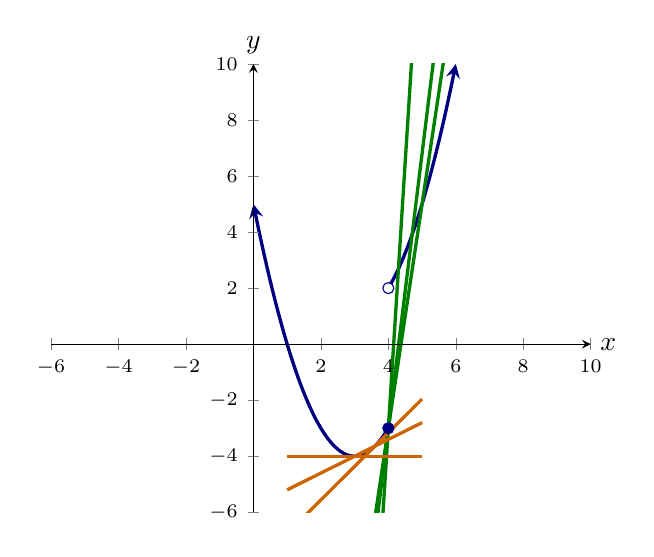
\begin{tikzpicture}
     \begin{axis}[
                domain=-10:10, ymax=10, xmax=10, ymin=-6, xmin=-6,
                axis lines =center, xlabel=$x$, ylabel=$y$,
                ytick={-6,-4,-2,2,4,6,8,10},
                xtick={-6,-4,-2,2,4,6,8,10},
                ticklabel style={font=\scriptsize},
                every axis y label/.style={at=(current axis.above origin),anchor=south},
                every axis x label/.style={at=(current axis.right of origin),anchor=west},
                axis on top,
                ]


        \addplot [draw=penColor, very thick, smooth, domain=(0:4),<-] {(x-3)^2 - 4};
        \addplot [draw=penColor, very thick, smooth, domain=(4:6),->] {(x-3)^2 + 1};

        \addplot [color=penColor,only marks,mark=*] coordinates{(4,-3)};
        \addplot [color=penColor,fill=white,only marks,mark=*] coordinates{(4,2)};
        
       


        \addplot [draw=penColor4, very thick, smooth, domain=(3:8)] {19*(x-4)-3};
        \addplot [draw=penColor4, very thick, smooth, domain=(3:8)] {9.8*(x-4)-3};
        \addplot [draw=penColor4, very thick, smooth, domain=(3:8)] {8*(x-4)-3};




        \addplot [draw=penColor5, very thick, smooth, domain=(1:5)] {-4};
        \addplot [draw=penColor5, very thick, smooth, domain=(1:5)] {0.6*(x-3.3)-3.82};
        \addplot [draw=penColor5, very thick, smooth, domain=(1:5)] {1.2*(x-3.6)-3.64};


       



    \end{axis}
\end{tikzpicture}
\end{image}

The two sides have tangent lines, but they are not smoothly turning to agree. \\


In this case, we say that there is no tangent line. \\

And, if there is no tangent line, then there is no slope of the tangent line, then the derivative has no value here. \\







So, a derivative implies that there are two sides and the two sides are agreeing. \\



But, there is no need to just throw everything else away.  We can extend our idea of derivative to include just one side. \\ 


























\begin{center}
\textbf{\textcolor{green!50!black}{ooooo-=-=-=-ooOoo-=-=-=-ooooo}} \\

more examples can be found by following this link\\ \link[More Examples of Quadratic Behavior]{https://ximera.osu.edu/csccmathematics/precalculus1/precalculus1/quadraticBehavior/examples/exampleList}

\end{center}




\end{document}




